\chapter{Data Simulation and Collection} \label{chapter:data}

\section{Introduction}
    
    ATLAS is responsible for collecting all the experimental data required for this analysis,
        but those data are of limited use without knowing how to interpret them.
    Without understanding how the key features of a physics interaction manifest within the electronics readout
        it is impossible to distinguish signal events from any other bunch crossing.
    Chapter \ref{chapter:theory} explained the theoretical motivation for this analysis.
    The past two chapters have focused entirely on the hardware necessary to produce and observe particle physics interactions.
    It falls on this chapter to describe how these two notions --
        mathematical equations and electronic circuits -- can be meshed into a single comparable concept.
    To compare the intangible and the physical on the same terms,
        one must enter the realm of software and digital data.

    This chapter will have to begin by backtracking slightly,
        describing the software analogs of the three chapters that have lead up to this point.
    These analogs will take the form of Monte-Carlo simulation frameworks
        that are collectively able to emulate the signals expected from the ATLAS hardware
        based on theoretical Lagrangians.
    Once the software description of physics processes is caught up,
        I can move forward in discussing what happens to the
        simulated and true electrical signals of ATLAS as they are read out.
    The real output bandwidth of ATLAS is extraordinary,
        so the simulated output is used to inform the usage of
        a rapid filtering mechanism called the trigger system.
    In turn, the simulated samples are processed by a simulation of this same trigger system,
        while the electrical signals are routed through the physical trigger system.
    The final output of both of these operations is identically formatted data files,
        which can be further refined and directly compared for the purpose of statistical analysis.
        

\FloatBarrier
\section{Monte-Carlo Simulation} \label{sec:mcsim}
    
    All of the remaining chapters of this thesis are in some way dependent on simulated event samples.
    Without a way to link pure physics equations to observable physical phenomena,
        there is no way to make meaningful decisions or predictions about collected data.
    Currently, Monte-Carlo simulation\cite{montecarlo} is among the most effective methods of making predictions
        for how theoretical parameters should affect experimental observations in particle physics\cite{compphys}.

    There are three core software frameworks used for this analysis,
        each corresponding to the three phases of interaction described in the prior chapters.
    The Lagrangian formalism, Feynman diagrams, and cross-section calculations of Chapter \ref{chapter:theory}
        are handled by a framework called MadGraph\cite{madgraph}.
    Showering, decay chains, and radiative processes follow in the immediate aftermath of
        hard-scatter events such as those at the interaction points of the LHC (Section \ref{sec:lhc-interaction_region}).
    These physical mechanisms are simulated by a pair of programs, Pythia8\cite{pythia} and EvtGen\cite{EvtGen}.
    As hadronic showers and ionizing particles pass through ATLAS (Chapter \ref{chapter:atlas})
        they cause a cascade of electrical signals and scattering effects.
    This highly complex set of interactions is modeled by the Geant4 framework\cite{geant4}.
    Collectively, these three programs are designed to
        generate a faithful reproduction of how a collection of \vbfhhproc events would appear,
        were they to occur in data collected from ATLAS.


    \subsection{MadGraph}

    Madgraph is technically a meta-code, a program that creates a program,
        with the created program designed to simulate physics in a prescribed manner.
    To do this, Madgraph needs a theory model, which consists of a Lagrangian of the desired physics
        alongside input parameters such as coupling values and particle masses.
    The Feynman rules are derived from the given Lagrangian,
        which are in turn used to create the process's matrix elements (see Section \ref{sec:feyn_rules}).
    Feynman rules alone are sufficient to then produce tree-level calculations automatically.
    For NLO calculations, additional counterterms must be supplied by hand
        so that matrix element computations appropriately converge during loop integrations. 
    With these features supplied, MadGraph generates code specific to the supplied model,
        which in turn calculates and computes the matrix elements of the requested process.
    A large number of events are produced using Monte Carlo techniques,
        each involving a different configuration of four momenta for the associated particles.
    These events represent a different point in the phase-space of the process,
        and a weight is assigned to each corresponding to its probability as calculated from the matrix element computation.
    The final collection of events is then output for use by later stages of the simulation process.

    \subsection{Pythia8 and EvtGen}\label{sec:pythia}

    The final particles produced by MadGraph are often short-lived and unstable,
        and so require further simulation of their evolution.
    Pythia8 and EvtGen are the software frameworks responsible for this phase of the simulation. 
    By default, Pythia8 is entirely self-contained, and can generate physics processes entirely on its own.
    However, the processes available to it are limited,
        hence the need to first generate the bare interaction with MadGraph.
    Pythia8 operates in three stages: process generation, partonic activity handling, and hadronization/decay.
    Process generation is the step which is taken over by MadGraph.
    The partonic stage addresses what happens to the parts of the proton \textit{not} involved in the immediate interaction (beam remnants),
        initial and final-state radiation of the final state particles, and inter-parton interactions.
    Following this is the hadronization stage, wherein final-state (but unstable)
        hadronic particles are extended through a cycle of radiation, decay, annihilation, and creation
        until a shower of stable hadronic matter remains.
    These steps are not fixed in Pythia's framework,
        and individual particles can transfer back and forth between these three stages
        as necessary to reach the stable state of the event as would be observed through a detector.
    Where Pythia8 falls short is in its simulation of longer lived hadrons,
        mainly B and D hadrons.
    Such hadrons are instead further simulated by EvtGen,
        which uses decay amplitudes of processes to determine the kinematic distributions
        of final state particles in an interaction.
    After hadronization, the emulation of the detector's response to these particles/partons
        then constitutes the final step of event simulation, which is handled by Geant4.
    

    \subsection{Geant4}

    Geant4 is a robust particle simulation framework
        that seeks to provide a comprehensive simulation of how particles behave as they propagate through physical materials.
    The entire geometry of the material in question is specified in the Geant4 framework in terms of
        its specific shape, location, and material properties.
    For this analysis, that means a replica of the entire ATLAS detector,
        down to the copper wiring and individual metal bolts,
        has been meticulously crafted across a set of specification files Geant4 can read in.
    After specifying the geometry to simulate, individual events can be propagated through the materials.

    An event procedure starts with a set of final-state particles,
        either generated through one of Geant4's built-in processes,
        or provided to it from an external program (in this case, Pythia8).
    These particles are moved forward in small time steps, according to their associated four-momentum.
    As they encounter different materials,
        these time steps are adjusted to be longer or shorter depending on
        the expected mean-free path and radiation length of the particle.
    For every step in a particle's movement,
        Geant4 examines a wide variety of physics processes the particle can undergo,
        ranging across material scattering, radiation, decay, and so on.
    Particles are split, absorbed, and created as necessary,
        until all particles have either been absorbed by material
        or exited the physical scope of the simulation (e.g.\ muons escaping from ATLAS).

    Geant4 additionally simulates the response of materials to these particle interactions,
        allowing energy and charge readouts to be simulated as they would be found within detector elements.
    The last step is to digitize these material responses so as to emulate the electrical signals of a real detector.
    All of the event response information, as well as an abundance of \textit{truth} information related to the simulated particles,
        is exported to a file format identical in content to that produced by the ATLAS trigger system.
    These simulated event samples can then be processed in the same manner as real data,
        allowing critical studies to be performed that in turn produce
        a far better understanding of the data's underlying physics.

    On a more immediately relevant note, these simulated events can be run through a variety of filtering algorithms,
        in order to test the utility of these algorithms and their parameters.
    These algorithms must be able to limit the throughput of events,
        without removing too many events of interest.
    Once a satisfactory level of performance is achieved these algorithms can be applied to the real ATLAS detector,
        in the form of the ATLAS trigger system.


\section{Trigger System} \label{sec:trigger}

    The amount of data output by the ATLAS detector is immense and overwhelming.
    Reading out every single bunch crossing would require phenomenal bandwidth and would take far too long to process.
    To counteract this overabundance of data, ATLAS relies on an on-site bunch crossing filtering system to drastically reduce the throughput.
    Known as the ATLAS trigger system, this critical piece of infrastructure constitutes the last step of data taking
        and the first step of physics analysis.

    The trigger system is a series of hardware- and software-level algorithms designed
        to quickly identify bunch crossing ``events'' which may be of interest to physics analysis,
        while discarding the rest.
    Referred to as ``online'' analysis, these algorithms perform event selection live,
        in parallel to the ATLAS detector observing collisions.
    The trigger system processes all ATLAS events immediately after readout,
        ultimately reducing the 40 MHz bunch crossing rate to a data output rate of 1 kHz.
    The data that survive this rapid selection are read out to disk
        and distributed to individual research teams for more sophisticated ``offline'' analysis later.

    \begin{figure}[h]
        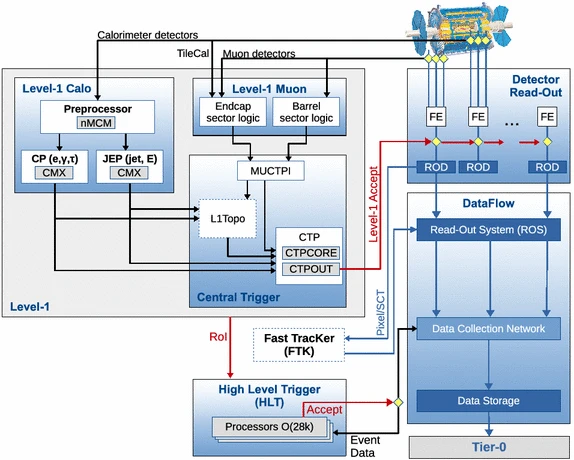
\includegraphics[width=\linewidth,height=\textheight,keepaspectratio]{trigger/trigger_flow}
        \caption{Flow chart of information through the ATLAS trigger system\cite{trigger_run2}.}
        \label{fig:trigger_flow}
    \end{figure}
    
    Triggering is achieved by running events through two sequential algorithmic systems.
    All events first go through the hardware-based Level 1 Trigger (L1) before being run through the more sophisticated (and slower) software-based High Level Trigger (HLT).
    Both of these systems involve a plethora of different measurements on various aspects of the events,
        such as total transverse energy, transverse momentum, jet multiplicity, and opening angles between jets
        (jets themselves are described in Section \ref{sec:jets}).
    All of these measurements are used, alone or in combination, to decide whether or not an event passes the trigger selection.

    Each of the various kinematic properties checked by the triggers have multiple threshold values that can determine a ``pass.''
    For example, a jet $p_T$ trigger can have thresholds at 30, 45, or 55 GeV, among others.
    A ``trigger chain'' is a combination of several different such kinematic conditions, each with their own thresholds.
    A bunch crossing is ultimately accepted and read out to disk for further analysis offline if it is able to pass all the conditions of a trigger chain.
    There are hundreds of different trigger chains, each permitting different combinations of kinematics,
        and each used by a variety of analyses targeting different processes.
    An event is read out if it passes any one of these trigger chains, and is labeled in data with all the trigger chains it passes.
    The trigger chains used in ATLAS were largely decided upon before the beginning of the Run 2 data taking period\footnote{
            Some trigger chains were introduced later, as the trigger menu can evolve mid-run.
        }, based on input from various analysis teams.
    This defined list of trigger chains comprise what is known as the ``trigger menu,'' and ultimately determines what kinds of physics processes ATLAS analyses have available.
    The following sections describe broadly how the two levels of the trigger system work, and later chapters will focus on which trigger menu items are used in the di-Higgs analysis specifically .

    \begin{figure}[h]
        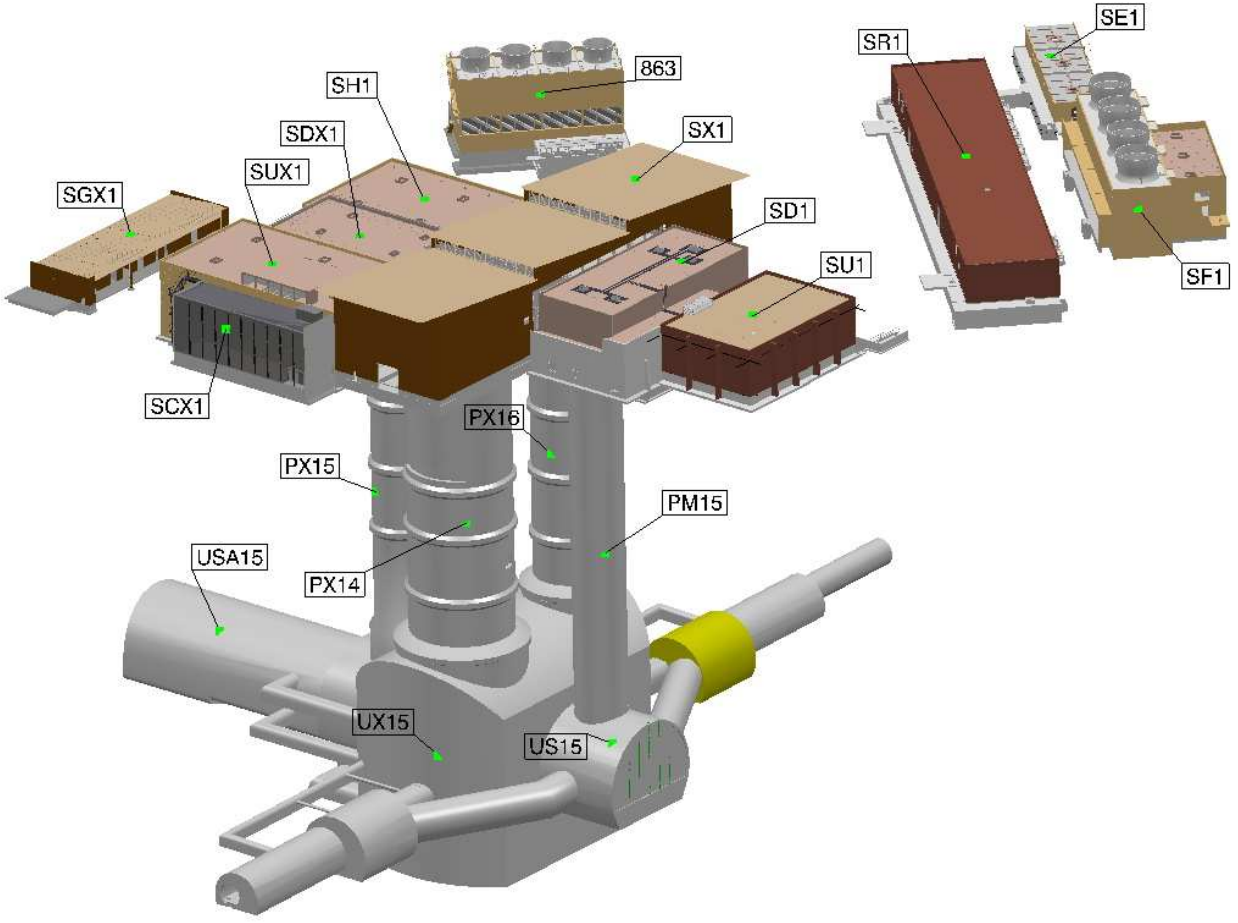
\includegraphics[width=\linewidth,height=\textheight,keepaspectratio]{trigger/facilities}
        \caption{General layout of buildings and facilities at LHC Point 1, site of ATLAS \cite{trigger_tdr}.}
        \label{fig:facilities}
    \end{figure}


    \subsection{Level 1 Trigger}\label{sec:L1}

        One bunch-crossing every 25 ns is a blistering operational pace.
        The first layer of the trigger system, L1, therefore must run entirely through hardware-level gate logic.
        The goal of this system is to reduce the event rate from the raw 40 MHz bunch-crossing rate,
            down to a more computationally manageable rate of 100 kHz \cite{trigger_run2}.
        To reduce latency as much as possible, all the electronics comprising L1 are located as close as possible to ATLAS itself, specifically in the USA15 underground chamber \cite{trigger_tdr} (see Fig. \ref{fig:facilities}).
        An additional consequence of the high L1 operating frequency
            is that it must exclusively use information from the ATLAS calorimeters and Muon Trigger Chamber for its decisions.
        %(utilizes detector buffer memory to keep up).

        The Muon Trigger aspect of L1 is based entirely on the dedicated Muon Trigger Chambers,
            described in section \ref{sec:muon-trigger_chamber}.
        Their purpose is to make trigger decisions primarily based on muon $p_T$ and track multiplicity\cite{trigger_run1}.
        In the calorimeter-based trigger, the selection algorithm first requires a reduction in data resolution.
        The full granularity of the ATLAS calorimeters is too high to analyze in the data collected so far by ATLAS\footnote{
            Though this is planned to change for the HL-LHC, which will have full granularity access at L1.
        }.
        Instead, the various sensors of the calorimeters are clustered together into ``trigger towers,''
            each with a resolution of $0.1 \times 0.1$ in $\Delta \eta \times \Delta \phi$.
        The way towers are clustered and used varies between the three different L1 calorimeter trigger modules.

        \begin{figure}[h] \centering
            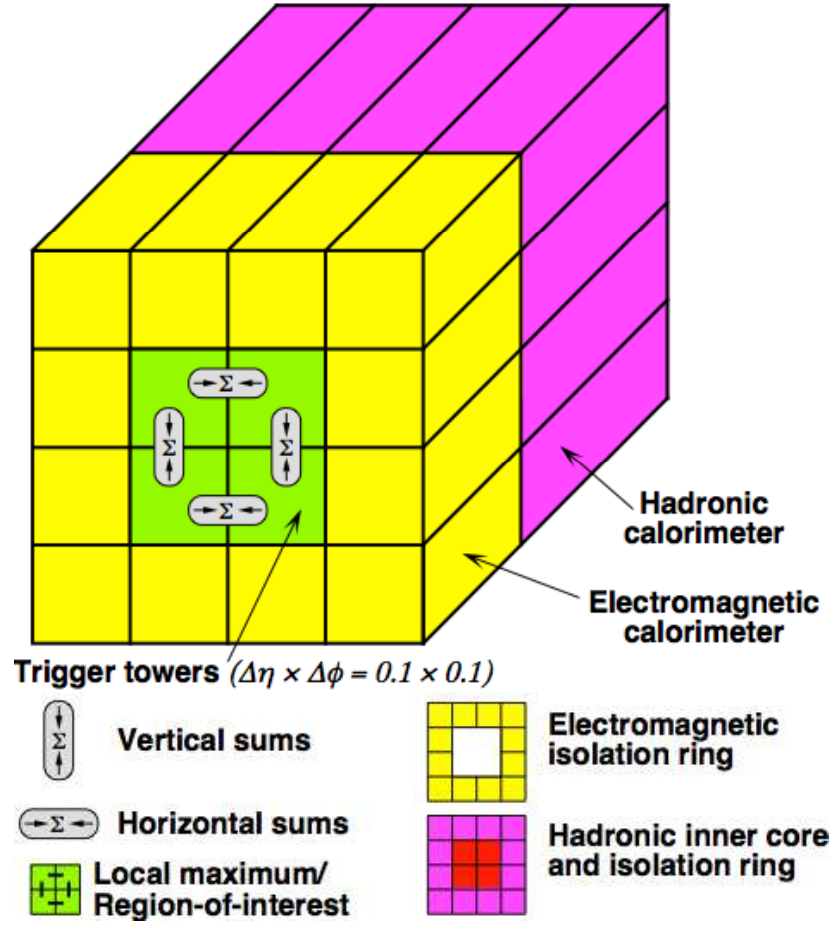
\includegraphics[width=\linewidth,height=0.4\textheight,keepaspectratio]{trigger/trigger_towers}
            \caption{Structure of trigger towers and Regions of Interest \cite{L1_calo_run1}.}
            \label{fig:trigger_towers}
        \end{figure}


        The Cluster Processor Module (CPM) exclusively uses the Barrel Calorimeters to function
            and is primarily meant for rapid identification of electrons/photons and taus/hadron jets.
        For either case, the CPM's first step is to check all possible $4 \times 4$ ``windows'' of trigger towers, identifying windows containing an isolated ``Region of Interest'' (RoI).
        Here, an RoI is defined as a $2 \times 2$ cluster of towers with an $E_T$ sum that is a relative maximum compared to surrounding towers.
        This $2 \times 2$ RoI is the center of the $4 \times 4$ window (see Fig. \ref{fig:trigger_towers}).
        Windows are considered as passing the CPM trigger if the RoI satisfies an isolation requirement,
            meaning that the 12 towers surrounding that core fall \textit{below} a predefined $E_T$ ``isolation threshold'' value.
        Electrons and photons are then separated from tau and hadronic jets by the fact that the latter group penetrates into the HCal barrel,
            while the former group stays highly contained to the ECal.

        Expanding out, the Jet/Energy Processing Module (JEM, or sometimes JEP) makes use of the calorimeter barrels and endcaps, as well as the FCAL, though it does not distinguish between the ECal and HCal.
        The JEM further reduces the granularity under consideration, with a basic unit of data collection being $2 \times 2$ collections of trigger towers called ``jet elements,'' resulting in a minimum resolution of $0.2 \times 0.2$ in $\Delta \eta \times \Delta \phi$.
        Like the CPM, the JEM runs its trigger conditions on windows of multiple jet elements that must be based around a $2 \times 2$ RoI core (which is a local $E_T$ maximum).
        Unlike the CPM, these windows can vary in size.
        Primarily, the JEM is intended to perform hit multiplicity counting
            as well as assist the Extended Cluster Merger Modules (CMX) in carrying out the final jet multiplicity
            and $E_T$ sums \cite{L1_calo_run1}\cite{trigger_run2}.
        When these conditions, alongside those performed in the Muon trigger, are completed, the event is passed along to the HLT.


\FloatBarrier
    \subsection{High Level Trigger}

        After the L1 Trigger has reduced the event rate to 100 kHz, the software-based High Level Trigger is used to further reduce the event rate to the final output of \textasciitilde 1 kHz.
        Located in the SCX1 building (Fig. \ref{fig:facilities}) at the surface of P1 (again to minimize latency),
            the HLT uses data from all detector elements to completely reconstruct the event as it occurred in ATLAS,
            and performs its selections based on this reconstructed event.
        Different physics processes and particles, known as physics ``signatures,'' are reconstructed in different ways
            and have different triggers based around them. 
        The main signatures used in ATLAS are:
            minimum bias signatures, electron/photons (Egamma), muons, jets, taus,
            missing transverse energy (MET), b-jets (as in jets from bottom quarks), and B-physics (as in B-hadrons).
        Reconstruction and selection within these signatures requires the use of highly technical algorithms
            which are further described in Chapters \ref{chapter:reconstruction} and \ref{chapter:selection}.
        Once events have successfully passed both L1 and the HLT, they are finally distributed off-site for analysis by different physics groups.

        \begin{figure}[h] \centering
            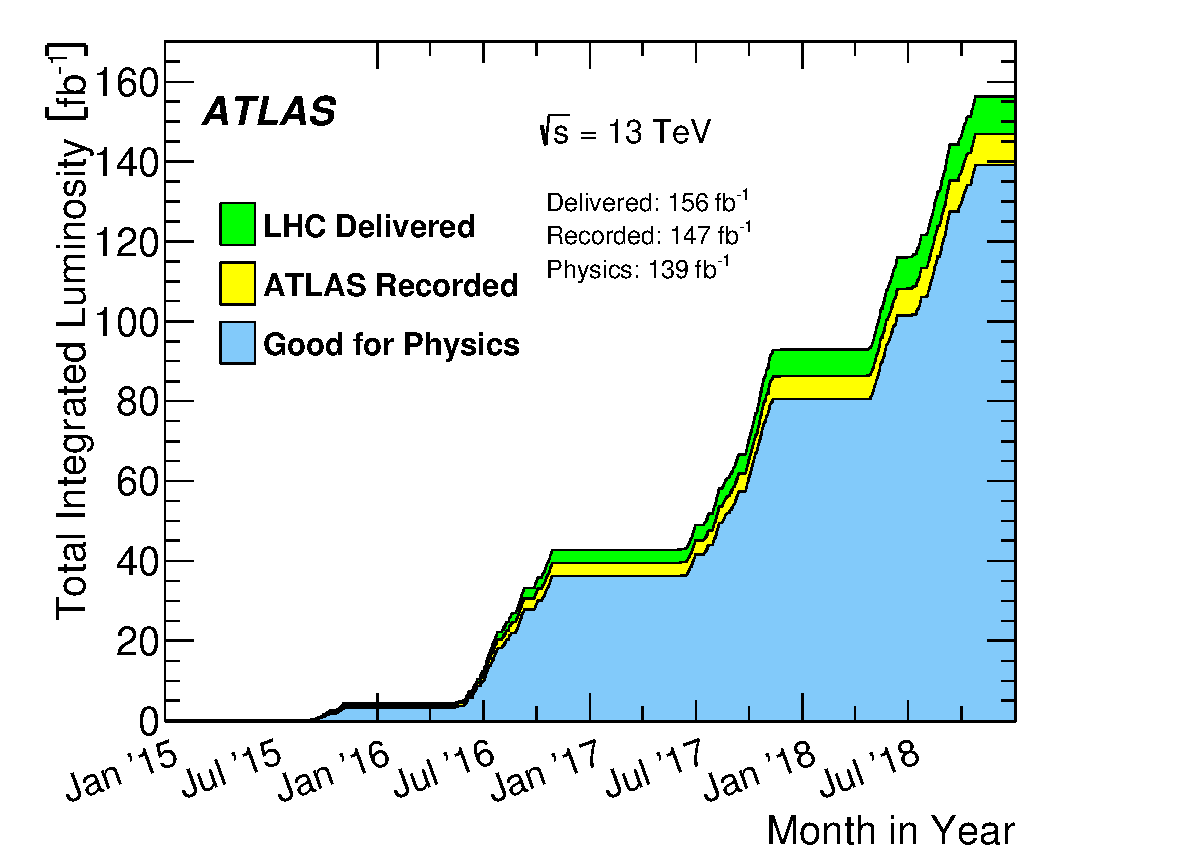
\includegraphics[width=\linewidth,height=0.4\textheight,keepaspectratio]{trigger/data_delivered}
            \caption{Amount of data collected, in terms of integrated luminosity,
                through the Run2 data taking period\cite{data_quality}.
                ``LHC Delivered'' refers to the amount of luminosity present during stable beams.
                ``ATLAS Recorded'' is luminosity that the ATLAS detector was active and recording for.
                ``Good for Physics'' describes all the luminosity that was actually able to be passed to offline storage,
                    as opposed to thrown out because of malfunctions or issues in ATLAS at the time.
            }
            \label{fig:data_delivered}
        \end{figure}

        Over its three operational years, Run 2 has resulted in a total of 139 \ifb of data which have passed the online triggers
            (see Fig. \ref{fig:data_delivered}).
        Due to an inefficiency in the vertex reconstruction present during 2016,
            only 125.9 \ifb of those data are actually used in my analysis.
        Nonetheless, with a wealth of both simulated and true events at last available, 
            physics analysis can now begin.
        On the one hand is a set raw electrical signals transmitted from the ATLAS circuitry.
        On the other is a collection of simulated signal events,
            wherein each event is tied through software back to its fundamental theoretical production mechanism.
        By recognizing the key features present in the simulated events,
            those same features can be identified in the true data.
        Data collection has now concluded, and it is time to begin the task of physics analysis,
            starting with reconstruction.
        %The first step of analysis is to recognize the key features present in the simulated data,
            %and then identify those same features in the true data in order to reconstruct the underlying physical objects.
